\documentclass[12pt]{article}
\usepackage[a4paper, total={6.5in, 10in}]{geometry}
\usepackage[test]{FunctionPlot}
\usepackage{MainTeX}
\usepackage{svg}


\title{宏包制作测试}
\author{Eureka}
\date{\today}

\begin{document}
\maketitle

\section{测试调用宏包时传递选项}
下面是宏包 {\ttfamily FunctionPlot}的一个选项(彩蛋):

\noindent\rule{.9\linewidth}{2pt}\\
\test


\section{测试宏包文本命令}
这个其实就是在之前的tcolorbox宏包中学到的样式,所以我就定义了这些彩色文本框: 
\Note{formal},\; \Note{tformal},\; \Note{warning},其实样式还是很简单的,目前就只有下面三个:
\begin{formal}{blue}
    没有标题的formal环境,自己定义颜色即可
\end{formal}

\begin{tformal}[blue]{Title}
    相比于formal环境,多了一个标题选项,所以这个环境也叫做tformal
\end{tformal}:

\begin{warning}
这个中间的内容就是警告
\end{warning}

\section{绘图命令}
自己在之前的命令基础上又重新定义了两个使用GNU Plot的绘图命令,
这样可以使得编译速度进一步加快。

\subsection{函数绘图}
至于普通的二三维的函数绘图十分简单的,你可以指定一下绘制的颜色,
或者说是colormap,定义域之类的plot parameters,尽情发挥。
下面我们主要绘制了 $y=x\sin(2x)$, $z=x*y$两个函数,效果还是可以的。

\begin{center}
    \Gplot[.9]{blue, domain=-12:12}{x*sin(2*x)}
    \Gplotz[.1]{bluered}{x*y}   

    \Gplotz[.1]{cool}{x*y}
\end{center}

\subsection{参数方程绘图}
主要是在vscode中定义了下面5个绘制命令的trigger
\begin{lstlisting}
trigger    --> 展开式
plot2d     --> \Gplot[scale]{color}{f(x)}
plot3d     --> \Gplotz[scale]{colormap style}{f(x, y)}
polarplot  --> \polarplot[scale][plot parameters]{f(\t)}
paraplot2d --> \paraplot[scale][plot parameters]{{x(t)},{y(t)}}
paraplot3d --> \paraplotz[scale][plot parameters]{{x(t)},{y(t)}}
\end{lstlisting}

其实参数方程作图主要就是\Note{极坐标},\Note{二维参数方程},
\Note{三维参数方程}这三种常见的情形.


那么我们就首先绘制极坐标的图形,下面我们绘制图形对应的方程分别为:
\begin{align}
    & \rho = \frac{0.01}{\pi \theta}\\
    & \rho = \sin(\theta)
\end{align}

\begin{formal}{red}
    只需要注意一下,就是polarplot,paraplot默认使用的是角度,而非弧度
\end{formal}

\begin{center}
    \polarplot[.7][red, domain=0:1440]{0.01/pi*\t}
    \polarplot[2][blue,thick,domain=0:120]{sin(\t)}
\end{center}


既然极坐标我们能够画出来了,那么接下来就是参数方程了,
\begin{center}
    \paraplot{{3*cos(t)}, {sin(t)}}
    \paraplot[.75][domain=1:2, orange, very thick]{{t}, {-2.5*(t-1.5)^2}}
\end{center}

最后就是我们的三维参数方程了,气质也是和上面的二维方程一样的,因为我们默认
$z(t) = t$,演示效果如下:下面我们绘制了螺旋线的方程 $x=\sin(t),y=3*\cos(t)(y=\cos(t)),z=t$
\begin{center}
    \paraplotz[.8]{{sin(t)}, {3*cos(t)}}
    \paraplotz[.8][blue,very thick,domain=0:1440]{{sin(t)}, {cos(t)}}
\end{center}



\section{图片插入}

其中有一个事情需要注意,由于svg的支持并不是很好,所以我没有把svg集成到
宏包中,想要调用svg矢量图,你需要安装了Inkscape,并且在导言区导入svg宏包。

\begin{figure}[!htb]
    \centering
    \includesvg[scale=.3]{./Doge.svg}
    \caption{主人公Doge图示}
    \label{Doge}
\end{figure}


\section{测试MMA}
同理,对应的MMA模块我也归纳到了FunctionPlot宏包中,
用于调用MMA生成对应的pdf矢量图片

\subsection{计算}
\begin{align}
    \wolfram{Series[Exp[x], {x, 0, 5}]}
\end{align}

\subsection{图片插入}
MMA 图片测试,下面的这个绘图还是比较复杂的,于是我们使用MMA绘制。

\begin{figure}[!htb]
    \centering
    \wolframgraphics{
		ContourPlot[
		x^2/4 + y^2/3 == 5, {x, -5, 5}, {y, -5, 5},
		ContourStyle->{
			% 同样的,被latex注释的部分不会传入MMA
			% RGBColor["\#00C0A3"], 
			% 在传参的过程中,不要使用#,即使是\#,MMA也是会报错的。
			RGBColor[0.,0.7529411764705882,0.6392156862745098],
			Thickness[0.004]
		},
		AspectRatio->1, 
		AxesOrigin->{0,0}, 
		Axes->True,
		Frame->False,
		AxesStyle->Arrowheads[{0, 0.03}],
		AxesLabel->{"x", "y"}
	]}{MMA2d1}
    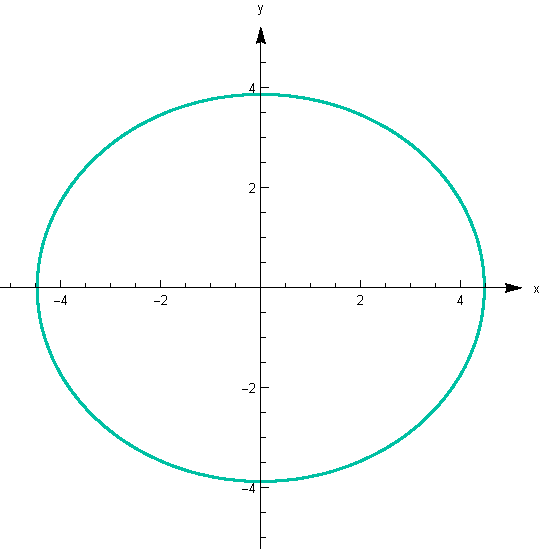
\includegraphics[scale=.7]{MMA2d1.pdf}
	\caption{MMA 二维图形}
	\label{MMA 二维图形}
\end{figure}

\begin{figure}[!htb]
    \centering
    \wolframgraphics{
    NumberLinePlot[
	    {Interval[{5, Infinity}], Interval[{2, 7}]}, 
	    AxesStyle->Arrowheads[{0, 0.03}]
    ]
    }{MMA2d2}
    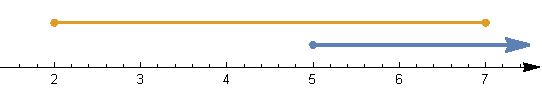
\includegraphics[scale=.7]{MMA2d2.pdf}
    \caption{MMA 二维图形2}
    \label{MMA 二维图形2}
\end{figure}

二维的一些图形绘制了之后,自然要去绘制一些MMA中的3维对象了。下面就是
一些例子:

\begin{figure}[!htb]
    \centering
    \wolframgraphics{
        Arrow[Tube[
		    BSplineCurve[{{0,0,0}, {.2,1,0.5},{2,1,1}}]
        ]]//Graphics3D}{MMA3d1}
    \wolframgraphics{
        VectorPlot3D[
            {x, y, z}, {x, -1, 1}, 
            {y, -1, 1}, {z,-1, 1},
            PlotTheme->"Classic"
        ]}{MMA3d2}
    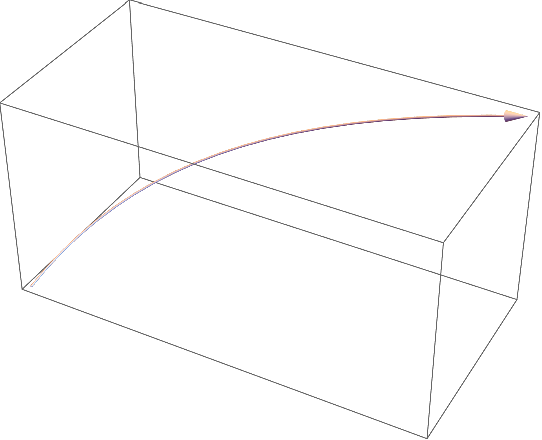
\includegraphics[scale=.7]{MMA3d1.pdf}
    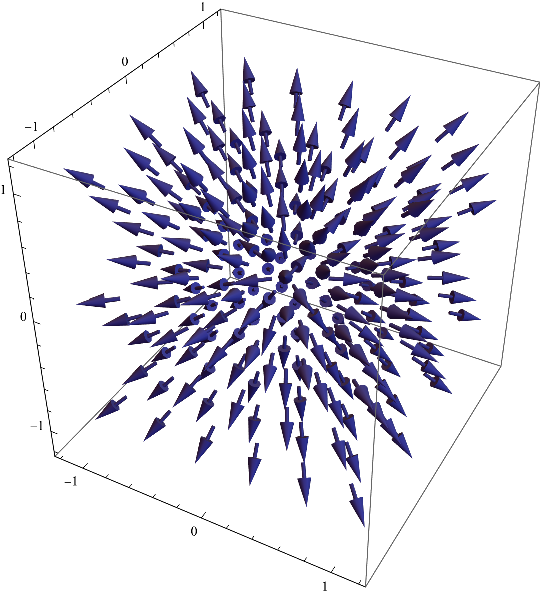
\includegraphics[scale=.7]{MMA3d2.pdf}
    \caption{MMA 三维图形}
    \label{MMA 三维图形}
\end{figure}


\subsection{表格功能}
MMA还能够解方程,微分方程,求根公式,输出表格等等.



\end{document}

